%Copyright 2004 by Till Tantau <tantau@users.sourceforge.net>.
%
% In principle, this file can be redistributed and/or modified under
% the terms of the GNU Public License, version 2.
%
% However, this file is supposed to be a template to be modified
% for your own needs. For this reason, if you use this file as a
% template and not specifically distribute it as part of a another
% package/program, I grant the extra permission to freely copy and
% modify this file as you see fit and even to delete this copyright
% notice. 

\documentclass{beamer}
\usepackage{braket}
\usepackage{mdframed}
\usepackage{multimedia}
\usepackage[export]{adjustbox}

% There are many different themes available for Beamer. A comprehensive
% list with examples is given here:
% http://deic.uab.es/~iblanes/beamer_gallery/index_by_theme.html
% You can uncomment the themes below if you would like to use a different
% one:
%\usetheme{AnnArbor}
%\usetheme{Antibes}
%\usetheme{Bergen}
%\usetheme{Berkeley}
%\usetheme{Berlin}
%\usetheme{Boadilla}
%\usetheme{boxes}
%\usetheme{CambridgeUS}
%\usetheme{Copenhagen}
%\usetheme{Darmstadt}
%\usetheme{default}
%\usetheme{Frankfurt}
%\usetheme{Goettingen}
%\usetheme{Hannover}
%\usetheme{Ilmenau}
%\usetheme{JuanLesPins}
%\usetheme{Luebeck}
\usetheme{Madrid}
%\usetheme{Malmoe}
%\usetheme{Marburg}
%\usetheme{Montpellier}
%\usetheme{PaloAlto}
%\usetheme{Pittsburgh}
%\usetheme{Rochester}
%\usetheme{Singapore}
%\usetheme{Szeged}
%\usetheme{Warsaw}
\title{Phase behaviour of the PSM GCM and GEM-$n$ models}

% A subtitle is optional and this may be deleted
\subtitle{Studied the softmatter physics with Monte Carlo}

\author{Yun-Hsuan Chou}
% - Give the names in the same order as the appear in the paper.
% - Use the \inst{?} command only if the authors have different
%   affiliation.

\institute[NTU] % (optional, but mostly needed)
{
	\inst{1}%
	Department of Pysics\\
	National Taiwan University
}

% - Use the \inst command only if there are several affiliations.
% - Keep it simple, no one is interested in your street address.

\date{Final Porject, 2016, 06, 26}
% - Either use conference name or its abbreviation.
% - Not really informative to the audience, more for people (including
%   yourself) who are reading the slides online

\subject{Studied the softmatter physics with Monte Carlo}
% This is only inserted into the PDF information catalog. Can be left
% out. 

% If you have a file called "university-logo-filename.xxx", where xxx
% is a graphic format that can be processed by latex or pdflatex,
% resp., then you can add a logo as follows:

% \pgfdeclareimage[height=0.5cm]{university-logo}{university-logo-filename}
% \logo{\pgfuseimage{university-logo}}

% Delete this, if you do not want the table of contents to pop up at
% the beginning of each subsection:
%\AtBeginSubsection[]
%{
%	\begin{frame}<beamer>{Outline}
%		\tableofcontents[currentsection,currentsubsection]
%	\end{frame}
%}

% Let's get started
\begin{document}

\begin{frame}
\titlepage
\end{frame}

\begin{frame}{Outline}
\tableofcontents
% You might wish to add the option [pausesections]
\end{frame}

% Section and subsections will appear in the presentation overview
% and table of contents.
\section{Introduction to the Monte Carlo Method}

\subsection{Demo - calculate $\pi$}

\begin{frame}{Introduction to the Monte Carlo Method}{Demo - calculate $\pi$}
\begin{itemize}
\item {
	Define a domain of the target.
	\begin{align}
		p(x,y) = \begin{cases}
			1 & \text{, } x^2 + y^2 \leq 1 \\
			0 & \text{, otherwise} 
		\end{cases}
	\end{align}
}
\item {
	Generate random numbers $(x_i, y_i)$ from uniform distribute $[-1, 1]$.
	\begin{align}	
		p_i = 1 \text{ if } &x^2+y^2 \leq 1\text{; } p+i = 0 \text{ otherwise} \\
		&\pi \approx \frac{1}{N} \sum_{i=1}^{N} pi + O( 1 / \sqrt{N})
	\end{align}
}
\end{itemize}
\end{frame}

\begin{frame}{Introduction to the Monte Carlo Method}{Demo - calculate $\pi$}
\end{frame}

\subsection{Demo - calculate 2-D classical Ising model}

\begin{frame}{Introduction to the Monte Carlo Method}{Demo - calculate 2-D classical Ising model}
	\begin{itemize}
		\item Build the configuration of a 2-D square lattice and set spins on each site. [Fig.~\ref{2DI}]
	\end{itemize}
	\begin{figure}[h]
		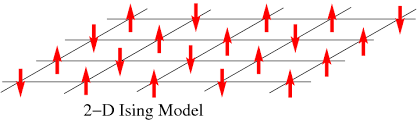
\includegraphics[width=0.50\textwidth]{figures/2DIsing.png}
		\label{2DI}
	\end{figure}
			\begin{align}
				&H = -J \sum_{i \neq j}{\sigma_i^z \sigma_j^z}\\ 
				&\Psi = \Ket{\sigma_1, \sigma_j, \cdots, \sigma_N}
			\end{align}
	\begin{itemize}
		\item Calculate the probability of the configuration at time $t$:
			\begin{align}
				P(E,t) =  e^{-\beta E(C)} \text{, where } \beta = \frac{1}{k_B T}
			\end{align}
	\end{itemize}

\end{frame}

\begin{frame}{Introduction to the Monte Carlo Method}{Demo - calculate 2-D classical Ising model}
	\begin{itemize}
		\item Importance Sampling: Metropolis algorithm \\

			Choose a spin randomly and determined that if it should be flipped to a new configuration $C^{\prime}$ \\
			\centerline{$\Delta E = E(C^{\prime}) - E(C)$}
			\begin{mdframed}
				\begin{align*}
					&\Delta E < 0 : \text{ accept filp} \\ 
					&\Delta E > 0 = \begin{cases}
					\text{accept }C^{\prime} \text{, if } e^{-\beta \Delta E} \geq \text{random number}  \\
					\text{reject }C^{\prime} \text{, otherwise} 
				\end{cases}
				\\
			\end{align*}
		\end{mdframed}
	\end{itemize}
\end{frame}

\begin{frame}{Introduction to the Monte Carlo Method}{Demo - calculate 2-D classical Ising model}
	\begin{columns}[c]
		\begin{column}[T]{4cm}
			\movie[height = 1.5 \textwidth, width = 1.0 \textwidth]{2D classical Ising}{figures/2DIsing.mpg}
		\end{column}
		\begin{column}[T]{8cm}
				\begin{figure}
					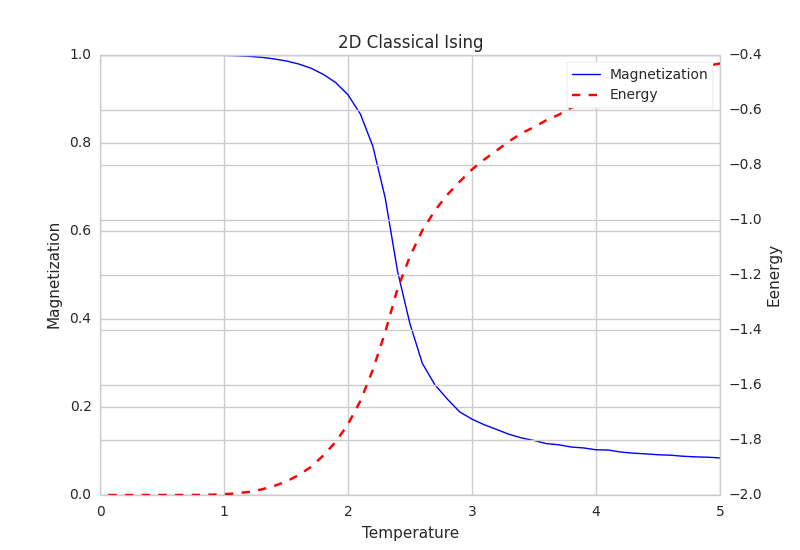
\includegraphics[width=0.9\textwidth]{figures/2DIsingEM.png}
					\label{2DI}
				\end{figure}
		\end{column}
	\end{columns}
\end{frame}

\begin{frame}{Introduction to the Monte Carlo Method}{Demo - calculate 2-D classical Ising model}
\end{frame}

\subsection{Calculate L-J particles in the NVT-ensemble}
% You can reveal the parts of a slide one at a time
% with the \pause command:
\begin{frame}{Introduction to the Monte Carlo Method}{Calculate L-J particlas in NVT ensemble}

\begin{itemize}
	\item Initialize a molecular configuration: \\
		In this case, we can set the atoms in the cubic sites.
	\item Determined the Trial move:
	\item Importance Sampling: Metropolis algorithm
	\item Repeat until the energy converge.
\end{itemize}
\end{frame}

\section{Introduction to the models for describing the phase behaviour}

\subsection{Penetrable Sphere Model (PSM) }
\subsection{Gaussian core Model (GCM) }
\subsection{Gaussian exponential Model (GEM-$n$)}

\begin{frame}{Introduction to the models for describing the phase behaviour}
	
\end{frame}

\section{Results}
\begin{frame}{Results}
	
\end{frame}

%\begin{frame}{Blocks}
%\begin{block}{Block Title}
%You can also highlight sections of your presentation in a block, with it's own title
%\end{block}
%\begin{theorem}
%There are separate environments for theorems, examples, definitions and proofs.
%\end{theorem}
%\begin{example}
%Here is an example of an example block.
%\end{example}
%\end{frame}
%
%% Placing a * after \section means it will not show in the
%% outline or table of contents.
%\section*{Summary}
%
%\begin{frame}{Summary}
%\begin{itemize}
%\item
%The \alert{first main message} of your talk in one or two lines.
%\item
%The \alert{second main message} of your talk in one or two lines.
%\item
%Perhaps a \alert{third message}, but not more than that.
%\end{itemize}
%
%\begin{itemize}
%\item
%Outlook
%\begin{itemize}
%\item
%Something you haven't solved.
%\item
%Something else you haven't solved.
%\end{itemize}
%\end{itemize}
%\end{frame}
%
%
%% All of the following is optional and typically not needed. 
%\appendix
%\section<presentation>*{\appendixname}
%\subsection<presentation>*{For Further Reading}
%
%\begin{frame}[allowframebreaks]
%\frametitle<presentation>{For Further Reading}
%
%\begin{thebibliography}{10}
%
%\beamertemplatebookbibitems
%% Start with overview books.
%
%\bibitem{Author1990}
%A.~Author.
%\newblock {\em Handbook of Everything}.
%\newblock Some Press, 1990.
%
%
%\beamertemplatearticlebibitems
%% Followed by interesting articles. Keep the list short. 
%
%\bibitem{Someone2000}
%S.~Someone.
%\newblock On this and that.
%\newblock {\em Journal of This and That}, 2(1):50--100,
%	2000.
%	\end{thebibliography}
%	\end{frame}

\end{document} 

